\documentclass[10pt]{article}

\usepackage[
    paperwidth=15cm,
    paperheight=24cm,
    top=1.0cm,
    bottom=4.0cm,
    left=1.0cm,
    right=4.0cm
]{geometry}

\usepackage{listings}
\usepackage{graphicx}

\lstset{
    basicstyle=\ttfamily\footnotesize,
    numbers=none,
    frame=none,
    keywordstyle=\normalfont,
    commentstyle=\normalfont,
    stringstyle=\normalfont,
    showstringspaces=false,
    breaklines=true,
    columns=flexible
}

\begin{document}

\noindent
Name: Dheeraj A G\\
Roll No: 25

\vspace{0.15cm}

\noindent
\makebox[\textwidth]{\dotfill}

\vspace{0.05cm}

\begin{center}
    \textbf{SIMULATION OF DETERMINISTIC FINITE AUTOMATA,DFA}
\end{center}

\vspace{0.05cm}

\noindent
\makebox[\textwidth]{\dotfill}

\vspace{0.15cm}

\noindent
\underline{\textbf{PROGRAM}}

\vspace{0.1cm}

\begin{lstlisting}
#include <stdio.h>
#include <string.h>

int main(){
    int n, m, i, j, current, fi, final[10], f, choice;
    char input[10], str[20], ch;
    int trans[10][10];

    printf("Enter number of states: ");
    scanf("%d", &n);

    printf("Enter number of input symbols: ");
    scanf("%d", &m);

    printf("Enter input symbols:\n");
    for(i = 0; i < m; i++){
        scanf(" %c", &input[i]);
    }

    printf("\nEnter transition table:\n");
    for(i = 0; i < n; i++){
        for(j = 0; j < m; j++){
            printf("delta(%d, %c) = ", i, input[j]);
            scanf("%d", &trans[i][j]);
        }
    }

    printf("Enter number of final states: ");
    scanf("%d", &fi);

    printf("Enter final states:\n");
    for(i = 0; i < fi; i++){
        scanf("%d", &final[i]);
    }

    do{
        printf("Enter input string: ");
        scanf("%s", str);

        current = 0;

        for(i = 0; i < strlen(str); i++){
            ch = str[i];

            for(j = 0; j < m; j++){
                if(ch == input[j]){
                    current = trans[current][j];
                    break;
                }
            }

            if(j == m){
                printf("Invalid input symbol\n");
                return 0;
            }
        }

        f = 0;

        for(i = 0; i < fi; i++){
            if(current == final[i])
            {
                f = 1;
                break;
            }
        }

        if(f)
            printf("Accepted\n");
        else
            printf("Rejected\n");

        printf("Enter your choice (0 - end, 1 - continue): ");
        scanf("%d", &choice);

    } while(choice == 1);

    return 0;
}
\end{lstlisting}

\newpage

\noindent
\underline{\textbf{OUTPUT}}

\vspace{0.1cm}

\noindent
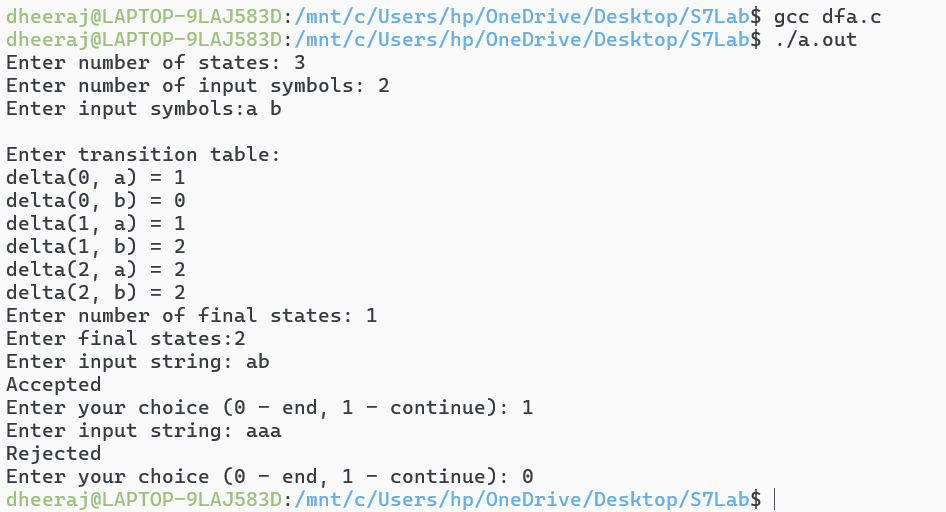
\includegraphics[width=\textwidth]{outs/exp1.png}

\newpage

\noindent
Name: Dheeraj A G\\
Roll No: 25

\vspace{0.15cm}

\noindent
\makebox[\textwidth]{\dotfill}

\vspace{0.05cm}

\begin{center}
    \textbf{ELIMINATION OF WHITE SPACES AND COMMENT LINES FROM A C PROGRAM}
\end{center}

\vspace{0.05cm}

\noindent
\makebox[\textwidth]{\dotfill}

\vspace{0.15cm}

\noindent
\underline{\textbf{PROGRAM}}

\vspace{0.1cm}

\begin{lstlisting}
#include <stdio.h>

void main(int argc, char *argv[]){
    FILE *fp1, *fp2;
    int ch, ch1, ch2;

    fp1 = fopen(argv[1], "r");
    fp2 = fopen(argv[2], "w");

    while ((ch = fgetc(fp1)) != EOF){
        switch (ch){
            case ' ':
            case '\t':
            case '\n':
                break;

            case '/':
                ch1 = fgetc(fp1);

                if (ch1 == '/'){

                    while ((ch = fgetc(fp1)) != '\n' && ch != EOF);
                }
                else if (ch1 == '*'){

                    while ((ch1 = fgetc(fp1)) != EOF){
                        if (ch1 == '*'){
                            ch2 = fgetc(fp1);

                            if (ch2 == '/')
                                break;
                            else
                                ungetc(ch2, fp1);
                        }
                    }
                }
                else{

                    fputc('/', fp2);

                    if (ch1 != EOF)
                        ungetc(ch1, fp1);
                }
                break;

            default:
                fputc(ch, fp2);
        }
    }
    fclose(fp1);
    fclose(fp2);
    printf("\nOutput file '%s' created successfully.\n", argv[2]);
}
\end{lstlisting}

\vspace{0.15cm}

\noindent
\underline{\textbf{INPUT FILE (test.c)}}

\vspace{0.1cm}

\begin{lstlisting}
#include <stdio.h>

int main() {
    // Single-line comment
    /*
     * Multi-line comment
     * Hello, World!
     */
    printf("Hello, World!\n");
    return 0;
}

\end{lstlisting}

\vspace{0.15cm}

\noindent
\underline{\textbf{OUTPUT FILE (op.c)}}

\vspace{0.1cm}

\begin{lstlisting}
#include<stdio.h>intmain(){printf("Hello,World!\n");return0;}
\end{lstlisting}

\vspace{0.15cm}

\noindent
\underline{\textbf{OUTPUT}}

\vspace{0.1cm}

\noindent
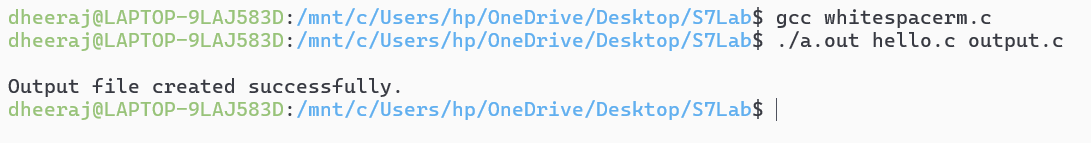
\includegraphics[width=\textwidth]{outs/exp2.png}

\newpage

\noindent
Name: Dheeraj A G\\
Roll No: 25

\vspace{0.15cm}

\noindent
\makebox[\textwidth]{\dotfill}

\vspace{0.05cm}

\begin{center}
    \textbf{IMPLEMENTATION OF LEXICAL ANALYZER IN C}
\end{center}

\vspace{0.05cm}

\noindent
\makebox[\textwidth]{\dotfill}

\vspace{0.15cm}

\noindent
\underline{\textbf{PROGRAM}}

\vspace{0.1cm}

\begin{lstlisting}
#include <stdio.h>
#include <stdlib.h>
#include <string.h>
#include <ctype.h>

void main(int argc, char *argv[]){
    FILE *fp1, *fp2;
    int ch, ch1, line = 1, si = 0, i, flag = 0;
    char lexeme[50];
    char keyword[20][50] = {
        "void", "int", "char", "float", "double",
        "if", "else", "for", "while", "return",
        "break", "continue", "printf", "scanf",
        "fopen", "fclose", "fgetc", "ungetc"
    };

    fp1 = fopen(argv[1], "r");
    fp2 = fopen(argv[2], "w");
    fprintf(fp2, "SLNO\tLEXEME\tLINE NO\n");

    while ((ch = fgetc(fp1)) != EOF){
        if (ch == ' ' || ch == '\t');
        else if (ch == '\n'){
            line++;
        }
        else if (ch == ';'){
            si++;
            fprintf(fp2, "\n%d\t%c\tsemi_colon\t%d", si, ch, line);
        }
        else if (ch == '(' || ch == '{' || ch == '['){
            si++;
            fprintf(fp2, "\n%d\t%c\topen_bracket\t%d", si, ch, line);
        }
        else if (ch == ')' || ch == '}' || ch == ']'){
            si++;
            fprintf(fp2, "\n%d\t%c\tclose_bracket\t%d", si, ch, line);
        }
        else if (ch == '+' || ch == '-' || ch == '*' || ch == '/' || ch == '%'){
            si++;
            fprintf(fp2, "\n%d\t%c\tarithmetic_operator\t%d", si, ch, line);
        }
        else if (ch == '&' || ch == ',' || ch == '.' || ch == '#'){
            si++;
            fprintf(fp2, "\n%d\t%c\tspecial_operator\t%d", si, ch, line);
        }
        else if (ch == '<' || ch == '>' || ch == '!'){
            i = 0;
            lexeme[i++] = ch;
            ch1 = fgetc(fp1);
            if (ch1 == '='){
                lexeme[i++] = ch1;
                lexeme[i] = '\0';
            }
            else{
                lexeme[i] = '\0';
                ungetc(ch1, fp1);
            }
            si++;
            fprintf(fp2, "\n%d\t%s\trelational_operator\t%d", si, lexeme, line);
        }
        else if (ch == '='){
            i = 0;
            ch1 = fgetc(fp1);
            if (ch1 == '='){
                lexeme[i++] = ch1;
                lexeme[i] = '\0';
                si++;
                fprintf(fp2, "\n%d\t%s\trelational_operator\t%d", si, lexeme, line);
            }
            else{
                lexeme[i] = '\0';
                ungetc(ch1, fp1);
                si++;
                fprintf(fp2, "\n%d\t%s\tassignment_operator\t%d", si, lexeme, line);
            }
        }
        else if (isdigit(ch)){
            flag = 0;
            i = 0;
            ch1 = ch;
            do{
                lexeme[i++] = ch1;
                if (ch1 == '.')
                {
                    flag = 1;
                }
                ch1 = fgetc(fp1);
            } 
            while (isdigit(ch1) || ch1 == '.');
            lexeme[i] = '\0';
            ungetc(ch1, fp1);
            if (flag == 1){
                si++;
                fprintf(fp2, "\n%d\t%s\tfloat_number\t%d", si, lexeme, line);
            }
            else{
                si++;
                fprintf(fp2, "\n%d\t%s\tnumber\t%d", si, lexeme, line);
            }
        }
        else if (isalpha(ch)){
            flag = 0;
            i = 0;
            ch1 = ch;
            do{
                lexeme[i++] = ch1;
                ch1 = fgetc(fp1);
            } 
            while (isdigit(ch1) || isalpha(ch1));
            lexeme[i] = '\0';
            ungetc(ch1, fp1);
            for (int j = 0; j < 19; j++){
                if (strcmp(lexeme, keyword[j]) == 0){
                    flag = 1;
                    break;
                }
            }
            if (flag == 1){
                si++;
                fprintf(fp2, "\n%d\t%s\tkeyword\t%d", si, lexeme, line);
            }
            else{
                si++;
                fprintf(fp2, "\n%d\t%s\tidentifier\t%d", si, lexeme, line);
            }
        }
        else
            fprintf(fp2,"error");
    }

    fclose(fp1);
    fclose(fp2);
    printf("\nOutput file created successfully.\n");
}
\end{lstlisting}

\vspace{0.15cm}

\noindent
\underline{\textbf{INPUT FILE (hello.c)}}

\vspace{0.1cm}

\begin{lstlisting}
#include <stdio.h>

int main() {
    // Single-line comment
    /*
     * Multi-line comment
     * Hello, World!
     */
    printf("Hello, World!\n");
    return 0;
}

\end{lstlisting}

\vspace{0.15cm}

\noindent
\underline{\textbf{OUTPUT FILE (lex.txt)}}

\vspace{0.1cm}

\begin{lstlisting}
SLNO	LEXEME	LINE NO

1	#	special_operator	1
2	include	identifier	1
3	<	relational_operator	1
4	stdio	identifier	1
5	.	special_operator	1
6	h	identifier	1
7	>	relational_operator	1  
8	int	keyword	3
9	main	identifier	3
10	(	open_bracket	3
11	)	close_bracket	3
12	{	open_bracket	3 
13	/	arithmetic_operator	4
14	/	arithmetic_operator	4
15	Single	identifier	4
16	-	arithmetic_operator	4
17	line	identifier	4
18	comment	identifier	4 
19	/	arithmetic_operator	5
20	*	arithmetic_operator	5 
21	*	arithmetic_operator	6
22	Multi	identifier	6
23	-	arithmetic_operator	6
24	line	identifier	6
25	comment	identifier	6 
26	*	arithmetic_operator	7
27	Hello	identifier	7
28	,	special_operator	7
29	World	identifier	7
30	!	relational_operator	7 
31	*	arithmetic_operator	8
32	/	arithmetic_operator	8 
33	printf	keyword	9
34	(	open_bracket	9 
35	Hello	identifier	9
36	,	special_operator	9
37	World	identifier	9
38	!	relational_operator	9 
39	n	identifier	9 
40	)	close_bracket	9
41	;	semi_colon	9 
42	return	keyword	10
43	0	number	10
44	;	semi_colon	10 
45	}	close_bracket	11 
\end{lstlisting}

\vspace{0.15cm}

\noindent
\underline{\textbf{OUTPUT}}

\vspace{0.1cm}

\noindent
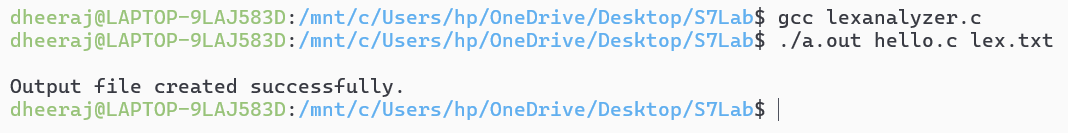
\includegraphics[width=\textwidth]{outs/exp3.png}

\newpage

\noindent
Name: Dheeraj A G\\
Roll No: 25

\vspace{0.15cm}

\noindent
\makebox[\textwidth]{\dotfill}

\vspace{0.05cm}

\begin{center}
    \textbf{IMPLEMENTATION OF RECURSIVE DESCENT PARSER}
\end{center}

\vspace{0.05cm}

\noindent
\makebox[\textwidth]{\dotfill}

\vspace{0.15cm}

\noindent
\underline{\textbf{PROGRAM}}

\vspace{0.1cm}

\begin{lstlisting}
#include <stdio.h>
#include <string.h>

char str[100];
int i =0,error =0;

void T(){
    if(str[i] =='a'){
        i++;
    }
    else{
        error=1;
    }
}

void X(){
    if(str[i] == '+'){
        i++;
        T();X();
    }
}

void E(){
    T();
    X();
}

int main(){
    printf("Enter the string:\n");
    scanf("%s",str);
    E();
    if(str[i] == '\0' && error ==0){
        printf("Accepted\n");
    }
    else{
        printf("Rejected\n");
    }
    return 0;
}


/*
E -> TX
T -> a
X -> +TX | epsilon
*/

\end{lstlisting}

\vspace{0.15cm}

\noindent
\underline{\textbf{OUTPUT}}

\vspace{0.1cm}

\noindent
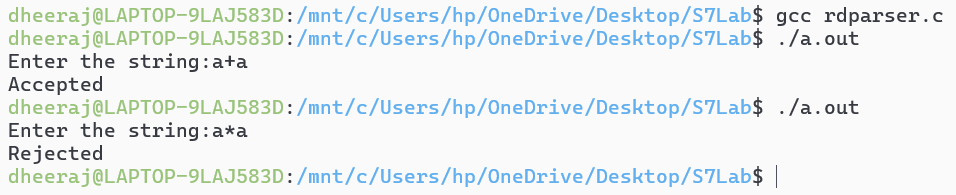
\includegraphics[width=\textwidth]{outs/exp4.png}

\newpage

\noindent
Name: Dheeraj A G\\
Roll No: 25

\vspace{0.15cm}

\noindent
\makebox[\textwidth]{\dotfill}

\vspace{0.05cm}

\begin{center}
    \textbf{IMPLEMENTATION OF OPERATOR PRECEDENCE PARSER}
\end{center}

\vspace{0.05cm}

\noindent
\makebox[\textwidth]{\dotfill}

\vspace{0.15cm}

\noindent
\underline{\textbf{PROGRAM}}

\vspace{0.1cm}

\begin{lstlisting}
#include <stdio.h>
#include <string.h>

#define MAX 20
#define STACK_SIZE 100

char table[MAX][MAX];
char terminals[MAX];
char stack[STACK_SIZE];

int n;
int top = -1;

int pos(char ch){
    for (int i = 0; i < n; i++)
    {
        if (terminals[i] == ch)
            return i;
    }
    return -1;
}

char topTerminal(){
    for (int i = top; i >= 0; i--)
    {
        if (stack[i] != 'E')
            return stack[i];
    }

    return '$';
}

void showStack(){
    for (int i = 0; i <= top; i++)
        printf("%c", stack[i]);
}

int valid(char handle[]){
    if (strcmp(handle, "i") == 0)
        return 1;

    if (strcmp(handle, "E+E") == 0)
        return 1;

    if (strcmp(handle, "E-E") == 0)
        return 1;

    if (strcmp(handle, "E*E") == 0)
        return 1;

    if (strcmp(handle, "E/E") == 0)
        return 1;

    if (strcmp(handle, "E^E") == 0)
        return 1;

    return 0;
}
int main(){
    char input[100];
    char handle[50];
    int ip = 0;
    int boundary, last;
    int len;
    int row, col;
    
    printf("Enter the no of terminals: ");
    scanf("%d", &n);
    
    printf("Enter the terminals: ");
    for (int i = 0; i < n; i++){
        scanf(" %c", &terminals[i]);
    }
    
    printf("\nEnter the precedence relation:\n");
    for (int i = 0; i < n; i++){
        for (int j = 0; j < n; j++){
            printf("%c & %c: ", terminals[i], terminals[j]);
            scanf(" %c", &table[i][j]);
        }
    }
    
    printf("\n\nOperator Precedence Table\n\n");
    printf("\t");
    for (int i = 0; i < n; i++)
        printf("%c\t", terminals[i]);
    printf("\n");
    for (int i = 0; i < n; i++){
        printf("%c\t", terminals[i]);
        for (int j = 0; j < n; j++){
            printf("%c\t", table[i][j]);
        }
        printf("\n");
    }
    
    printf("\nEnter the input string: ");
    scanf("%s", input);
    
    if (input[strlen(input) - 1] != '$')
        strcat(input, "$");
   
    top = -1;
    stack[++top] = '$';

    printf("\n%-15s %-15s %s\n","Stack", "Input", "Action");
    while (1){
        char a = topTerminal();
        char b = input[ip];
        
        if (top == 1 && stack[0] == '$' && stack[1] == 'E' && b == '$'){
            showStack();
            printf("\t\t%-15s\tAccept\n",input + ip);
            printf("\nACCEPTED.\n");
            break;
        }
        row = pos(a);
        col = pos(b);
        
        if (row == -1 || col == -1){
            printf("\nInvalid terminal encountered.\n");
            printf("REJECTED.\n");
            break;
        }
        
        if (table[row][col] == '<' || table[row][col] == '='){
            showStack();
            printf("\t\t%-15s\tShift %c\n",input + ip,b);

            stack[++top] = b;
            ip++;
        }
        
        else if (table[row][col] == '>'){
            last = -1;
            boundary = -1;
            for (int i = top; i >= 0; i--){
                if (stack[i] != 'E'){
                    if (last != -1){
                        int r1 = pos(stack[i]);
                        int r2 = pos(stack[last]);
                        if (r1 != -1 &&
                            r2 != -1 &&
                            table[r1][r2] == '<')
                        {
                            boundary = i;
                            break;
                        }
                    }

                    last = i;
                }
            }
            len = 0;
            for (int i = boundary + 1; i <= top; i++){
                handle[len++] = stack[i];
            }
            handle[len] = '\0';
            showStack();
            printf("\t\t%-15s\tReduce %s\n",input + ip,handle);
            
            if (!valid(handle)){
                printf("\nInvalid handle: %s\n", handle);
                printf("REJECTED.\n");

                return 0;
            }
            top = boundary;
            stack[++top] = 'E';
        }
        else{
            printf("\nNo valid precedence relation between %c and %c.\n",
                   a, b);

            printf("REJECTED.\n");
            break;
        }
    }
    return 0;
}
\end{lstlisting}

\newpage

\noindent
\underline{\textbf{OUTPUT}}

\vspace{0.1cm}

\noindent
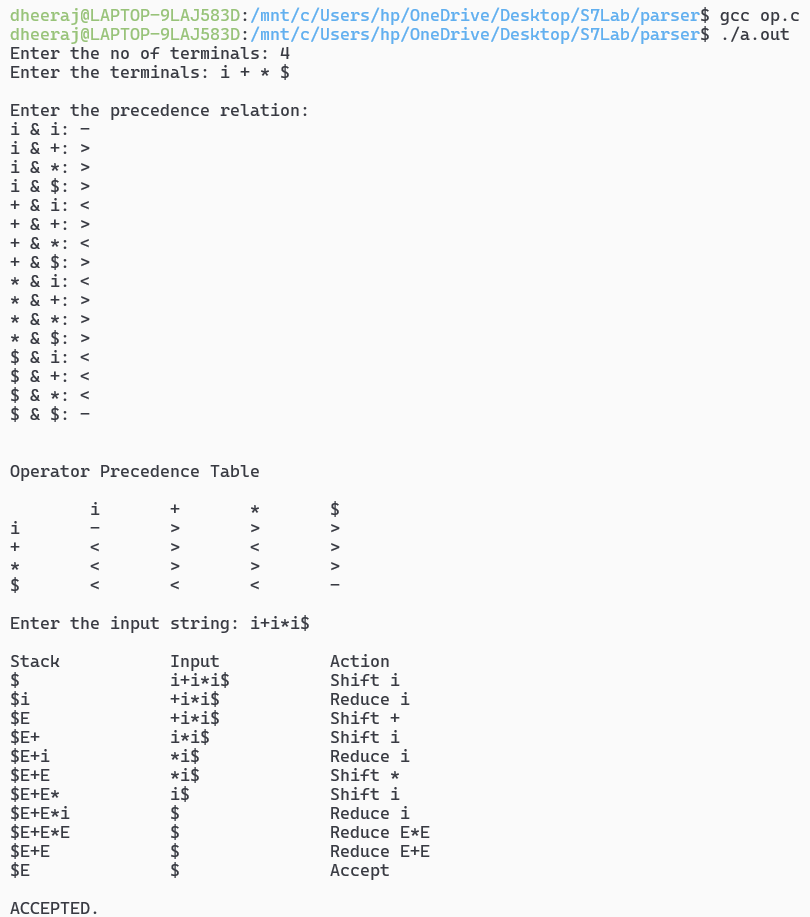
\includegraphics[width=\textwidth]{outs/exp5.png}

\vspace{0.15cm}

\noindent
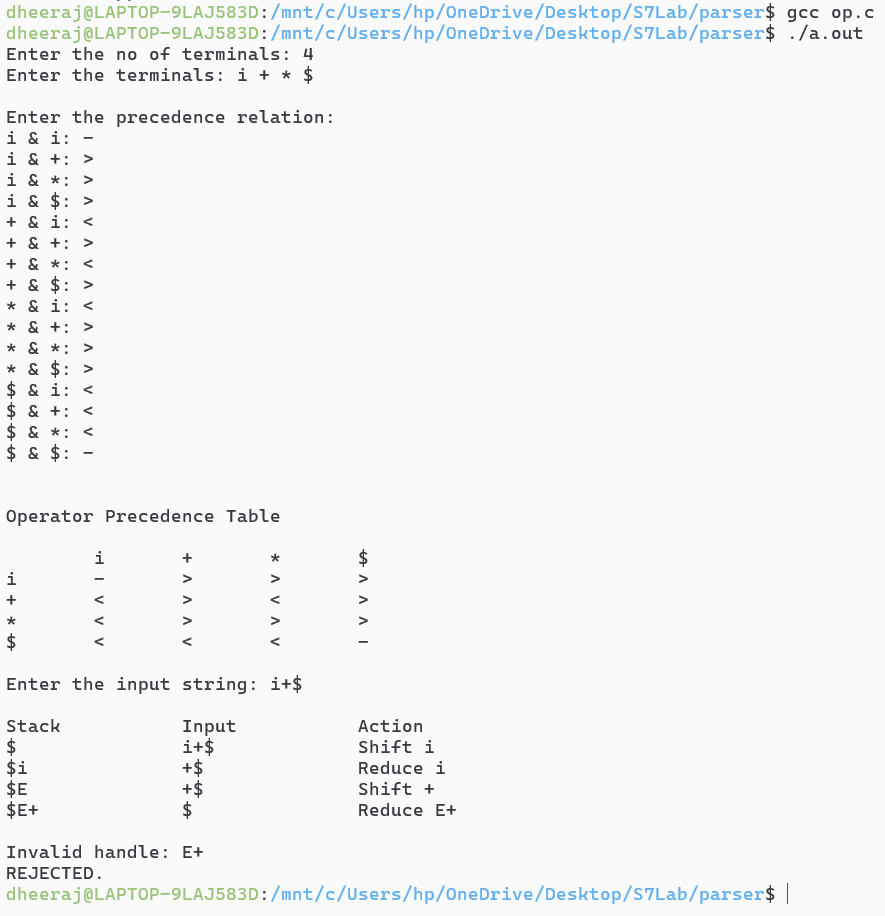
\includegraphics[width=\textwidth]{outs/exp5(2).png}

\newpage

\noindent
Name: Dheeraj A G\\
Roll No: 25

\vspace{0.15cm}

\noindent
\makebox[\textwidth]{\dotfill}

\vspace{0.05cm}

\begin{center}
    \textbf{CHECK FOR BALANCED PARENTHESES IN A C PROGRAM}
\end{center}

\vspace{0.05cm}

\noindent
\makebox[\textwidth]{\dotfill}

\vspace{0.15cm}

\noindent
\underline{\textbf{PROGRAM}}

\vspace{0.1cm}

\begin{lstlisting}
#include <stdio.h>
#include <stdlib.h>

#define MAX 100

typedef struct {
    char ch;
    int line;
} StackItem;

StackItem stack[MAX];
int top = -1;

StackItem pop(void) {
    StackItem empty = {'\0', 0};
    if (top == -1) {
        return empty;
    }
    return stack[top--];
}

void push(char val, int lineNo) {
    if (top == MAX - 1) {
        printf("Stack Overflow\n");
        return;
    }
    stack[++top].ch = val;
    stack[top].line = lineNo;
}

int main(int argc, char *argv[]) {
    FILE *file;
    char ch;
    int line = 1;
    int error = 0;

    if (argc != 2) {
        printf("Usage: %s <expression>\n", argv[0]);
        return 1;
    }

    file = fopen(argv[1], "r");
    if (file == NULL) {
        printf("Error opening file: %s\n", argv[1]);
        return 1;
    }
    printf("I am Dheeraj A G. Here is my output for parenthesis matching\n");
    while ((ch = fgetc(file)) != EOF) {
        if (ch == '\n') {
            line++;
            continue;
        }

        if (ch == '(' || ch == '{' || ch == '[') {
            push(ch, line);
        }
        else if (ch == ')' || ch == '}' || ch == ']') {
            if (top == -1) {
                printf("Right %c missing : Identified at line number %d\n", ch, line);
                error = 1;
            } else {
                StackItem item = pop();
                if ((ch == ')' && item.ch != '(') || (ch == '}' && 
                    item.ch != '{') || (ch == ']' && item.ch != '[')) {
                    printf("Parentheses mismatch between %c and %c : 
                            Identified at line number %d\n", item.ch, ch, line);
                    error = 1;
                }
            }
        }
    }

    while (top != -1) {
        StackItem item = pop();
        printf("Left %c missing : Identified at line number %d\n", item.ch, item.line);
        error = 1;
    }

    if (!error) {
        printf("Parentheses are balanced.\n");
    }

    fclose(file);
    return 0;
}

\end{lstlisting}

\vspace{0.15cm}

\noindent
\underline{\textbf{INPUT FILE (program.c)}}
\vspace{0.1cm}

\begin{lstlisting}
#include <stdio.h>
#define MAX 1000
int main(void {
    char expression[MAX];
    char stack[MAX];
    int top = -1;
    int balanced = 1;
    printf("Enter an expression: ");
    if (fgets(expression, sizeof(expression), stdin) == NULL) {
        return 1;
    for (int i = 0; expression[i != '\0'; ++i) {
        char ch = expression[i];
        if (ch == '(' || ch == '[' || ch == '{') {
            stack[++top] = ch;
        } else if (ch == ')' || ch == ']' || ch == '}') {
            if (top < 0 ||
                (ch == ')' && stack[top] != '(') ||
                (ch == ']' && stack[top] != '[') ||
                (ch == '}' && stack[top] != '{')) {
                balanced = 0;
                break;
            }
        
    }
    if (top != -1) {
        balanced = 0;
    }
    printf("%s\n", balanced ? "Parentheses are balanced." : "Parentheses are mismatched."};
    return 0;
}
\end{lstlisting}

\newpage

\noindent
\underline{\textbf{OUTPUT}}

\vspace{0.1cm}

\noindent
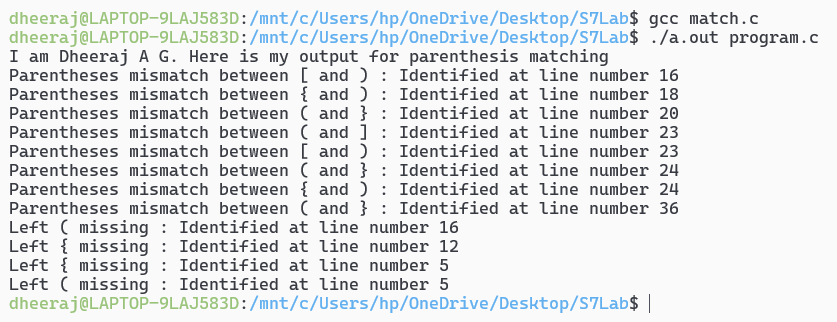
\includegraphics[width=\textwidth]{outs/exp6.png}

\newpage

\noindent
Name: Dheeraj A G\\
Roll No: 25

\vspace{0.15cm}

\noindent
\makebox[\textwidth]{\dotfill}

\vspace{0.05cm}

\begin{center}
    \textbf{FOR LOOP SYNTAX CHECKER IN C}
\end{center}

\vspace{0.05cm}

\noindent
\makebox[\textwidth]{\dotfill}

\vspace{0.15cm}

\noindent
\underline{\textbf{PROGRAM}}

\vspace{0.1cm}

\begin{lstlisting}
#include <stdio.h>
#include <stdlib.h>
#include <string.h>
#include <ctype.h>

int main(int argc, char *argv[]){
    FILE *fp;
    char line[500];
    char *p;
    int found = 0;
    int forno = 0;

    printf("Hi I'm Dheeraj A G.Here is my output for loop syntax checking.\n\n");
    if (argc < 2){
        printf(" Input file not specified.\n");
        printf(" %s <input_file>\n", argv[0]);
        return 1;
    }
    fp = fopen(argv[1], "r");

    if (fp == NULL){
        printf("Cannot open file '%s'.\n", argv[1]);
        return 1;
    }

    while (fgets(line, sizeof(line), fp) != NULL){
        p = line;

        while ((p = strstr(p, "for")) != NULL){
            if ((p == line || !isalnum(*(p - 1))) &&
                !isalnum(*(p + 3)) && *(p + 3) != '_'){
                int semicolon = 0;
                int open = 0;
                int close = 0;
                int error = 0;
                int i;

                found = 1;
                forno++;

                printf("for loop %d:", forno);

                p = p + 3;

                while (isspace(*p))
                    p++;

                /* Check '(' */
                if (*p != '('){
                    printf(" '(' is missing after 'for'.\n");
                    error = 1;

                    p++;
                    printf("\n");
                    continue;
                }

                open = 1;
                p++;

                for (i = 0; p[i] != '\0'; i++){
                    if (p[i] == ';')
                        semicolon++;

                    if (p[i] == '(')
                        open++;

                    if (p[i] == ')'){
                        open--;

                        if (open == 0){
                            close = 1;
                            break;
                        }
                    }
                }
                if (!close){
                    printf(" ')' is missing.\n");
                    error = 1;
                }
                if (semicolon != 2){
                    printf("  Expected 2 semicolons inside "
                           "'for' brackets, found %d.\n",
                           semicolon);
                    error = 1;
                }

                if (!error){
                    printf("  For loop syntax is OK.\n");
                }

                printf("\n");
            }

            p = p + 3;
        }
    }

    fclose(fp);
    if (!found)
        printf("'for' loop is not present.\n");

    return 0;
}


\end{lstlisting}

\vspace{0.15cm}

\noindent
\underline{\textbf{INPUT FILE (program.c)}}

\vspace{0.1cm}

\begin{lstlisting}
#include <stdio.h>

int main()
{
    int i;

    /* 1. Missing '(' */
    for i = 0; i < 10; i++)
    {
        printf("%d", i);
    }

    /* 2. Missing ')' */
    for(i = 0; i < 10; i++
    {
        printf("%d", i);
    }

    /* 3. Missing semicolon */
    for(i = 0; i < 10 i++)
    {
        printf("%d", i);
    }

    /* 4. Only one semicolon */
    for(i = 0; i < 10)
    {
        printf("%d", i);
    }

    /* 5. More than two semicolons */
    for(i = 0; i < 10; i++; i++)
    {
        printf("%d", i);
    }

    /* 6. Correct for loop */
    for(i = 0; i < 10; i++)
    {
        printf("%d", i);
    }
return 0;
}
\end{lstlisting}

\vspace{0.15cm}

\noindent
\underline{\textbf{OUTPUT}}

\vspace{0.1cm}

\noindent
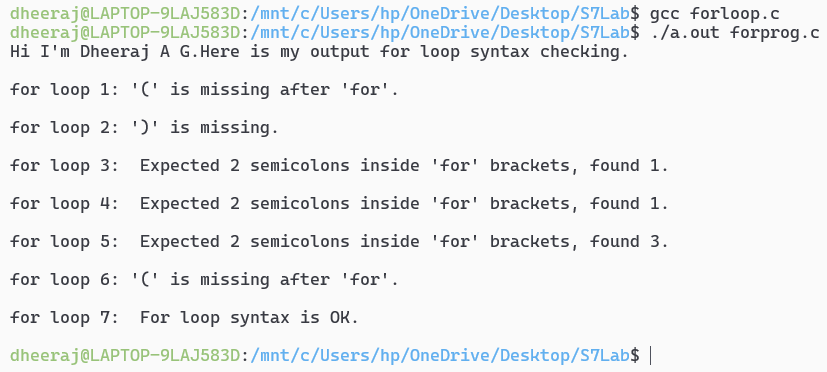
\includegraphics[width=\textwidth]{outs/exp7.png}

\newpage

\noindent
Name: Dheeraj A G\\
Roll No: 25

\vspace{0.15cm}

\noindent
\makebox[\textwidth]{\dotfill}

\vspace{0.05cm}

\begin{center}
    \textbf{IMPLEMENTATION OF SHIFT REDUCE PARSER}
\end{center}

\vspace{0.05cm}

\noindent
\makebox[\textwidth]{\dotfill}

\vspace{0.15cm}

\noindent
\underline{\textbf{PROGRAM}}

\vspace{0.1cm}

\begin{lstlisting}
/*
   Grammar:
   E -> E+E
   E -> E*E
   E -> (E)
   E -> i
*/

#include <stdio.h>
#include <string.h>

int main(void)
{
    char inp[21];
    char stack[50] = "";
    const char *left[] = {"E", "E", "E", "E"};
    const char *right[] = {"E+E", "E*E", "(E)", "i"};
    size_t posi = 0;
    int reduced;

    printf("I am Dheeraj A G. Here is my shift reduce parser output\n");
    printf("\nProductions are: \n");
    printf("E → E+E ∣ E∗E ∣ (E) ∣ i\n");
    printf("\nEnter the inp string: ");

    if (scanf("%19s", inp) != 1)
        return 1;

    strcat(inp, "$ ");
    inp[strlen(inp) - 1] = '\0';

    printf("Stack\tinp\tAction\n");

    while (posi < strlen(inp) - 1) {
        size_t stklen;
        char shifted[2] = {inp[posi++], '\0'};

        strcat(stack, shifted);
        printf("%s\t%s\tShift %s\n", stack,
               inp + posi, shifted);

        do {
            reduced = 0;
            stklen = strlen(stack);

            for (int rule = 0; rule < 4; rule++) {
                size_t rilen = strlen(right[rule]);

                if (stklen >= rilen &&
                    strcmp(stack + stklen - rilen, right[rule]) == 0) {
                    stack[stklen - rilen] = '\0';
                    strcat(stack, left[rule]);
                    printf("%s\t%s\tReduce %s->%s\n", stack,
                           inp + posi, left[rule], right[rule]);
                    reduced = 1;
                    break;
                }
            }
        } while (reduced);
    }

    do {
        reduced = 0;
        size_t stklen = strlen(stack);

        for (int rule = 0; rule < 4; rule++) {
            size_t rilen = strlen(right[rule]);

            if (stklen >= rilen &&
                strcmp(stack + stklen - rilen, right[rule]) == 0) {
                stack[stklen - rilen] = '\0';
                strcat(stack, left[rule]);
                printf("%s\t%s\tReduce %s->%s\n", stack,
                       inp + posi, left[rule], right[rule]);
                reduced = 1;
                break;
            }
        }
    } while (reduced);

    if (strcmp(stack, "E") == 0)
        printf("\nAccepted\n");
    else
        printf("\nNot Accepted\n");

    return 0;
}


\end{lstlisting}

\vspace{0.15cm}

\noindent
\underline{\textbf{OUTPUT}}

\vspace{0.1cm}

\noindent
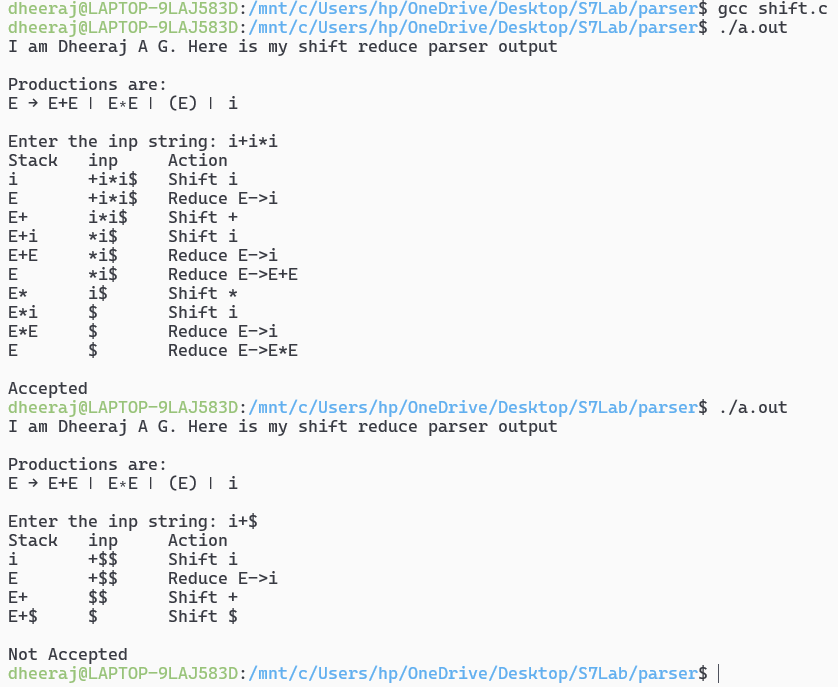
\includegraphics[width=\textwidth]{outs/exp8.png}

\newpage

\noindent
Name: Dheeraj A G\\
Roll No: 25

\vspace{0.15cm}

\noindent
\makebox[\textwidth]{\dotfill}

\vspace{0.05cm}

\begin{center}
    \textbf{IMPLEMENTATION OF LEXICAL ANALYZER USING LEX PROGRAM}
\end{center}

\vspace{0.05cm}

\noindent
\makebox[\textwidth]{\dotfill}

\vspace{0.15cm}

\noindent
\underline{\textbf{PROGRAM}}

\vspace{0.1cm}

\begin{lstlisting}
%{
    #include<stdio.h>
    int line = 1;
    int slno = 1;
%}
DIGIT [0-9]
ALPHA [a-zA-Z]
WS [ \t]
%%
{WS}+ {}
"\n" {line++;}
"void"|"main"|"if"|"else" {printf("\n%d\t%s\tkeyword\t%d",slno,yytext,line);slno++;}
{ALPHA}({ALPHA}|{DIGIT})* {printf("\n%d\t%s\tidentifier\t%d",slno,yytext,line);slno++;}
"+"|"-"|"*"|"/" {printf("\n%d\t%s\tarithmetic_op\t%d",slno,yytext,line);slno++;}
"<"|"<="|">"|">=" {printf("\n%d\t%s\trelop\t%d",slno,yytext,line);slno++;}
{DIGIT}+"."{DIGIT} {printf("\n%d\t%s\tfloat\t%d",slno,yytext,line);slno++;}
{DIGIT}+ {printf("\n%d\t%s\tnumber\t%d",slno,yytext,line);slno++;}
";" {printf("\n%d\t%s\tsemicolon\t%d",slno,yytext,line);slno++;}
"#"|"->"|"$" {printf("\n%d\t%s\tspecial\t%d",slno,yytext,line);slno++;}
. {printf("\n%d\t%s\tunrecognized\t%d",slno,yytext,line);slno++;}
%%
void main(int argc,char* argv[]){
    yyin=fopen(argv[1],"r");
    printf("slno\tlexeme\ttoken\tlineno");
    yylex();
    printf("\n");
}
int yywrap(){
    return 1;
}
\end{lstlisting}

\vspace{0.15cm}

\noindent
\underline{\textbf{INPUT FILE (hello.c)}}

\vspace{0.1cm}

\begin{lstlisting}
#include <stdio.h>

int main() {
    // Single-line comment
    /*
     * Multi-line comment
     * Hello, World!
     */
    printf("Hello, World!\n");
    return 0;
}

\end{lstlisting}

\newpage

\noindent
\underline{\textbf{OUTPUT}}

\vspace{0.1cm}

\noindent
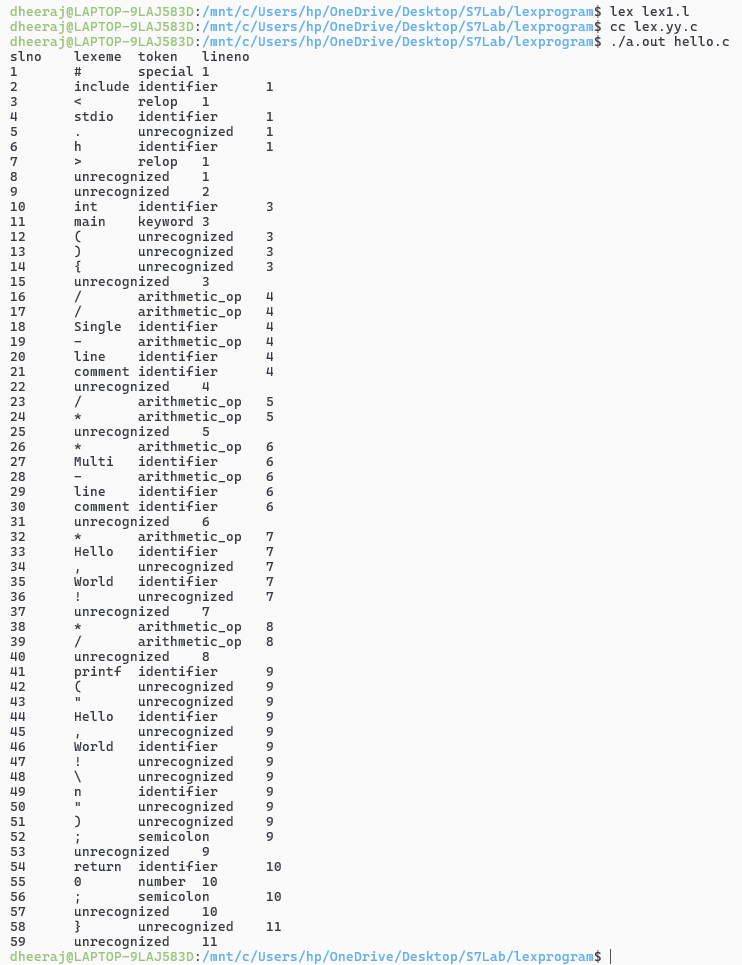
\includegraphics[width=\textwidth]{outs/exp9.png}

\newpage

\noindent
Name: Dheeraj A G\\
Roll No: 25

\vspace{0.15cm}

\noindent
\makebox[\textwidth]{\dotfill}

\vspace{0.05cm}

\begin{center}
    \textbf{SIMPLE CALCULATOR USING LEX PROGRAM}
\end{center}

\vspace{0.05cm}

\noindent
\makebox[\textwidth]{\dotfill}

\vspace{0.15cm}

\noindent
\underline{\textbf{PROGRAM}}

\vspace{0.1cm}

\begin{lstlisting}
%{
    #include <stdio.h>
    #include <stdlib.h>

    int result = 0;
    char operation = '+';
    int have_number = 0;
    int error = 0;

    void reset_calculator(void) {
        result = 0;
        operation = '+';
        have_number = 0;
        error = 0;
    }
%}
DIGIT [0-9]
%%
"+"|"-"|"*"|"/" {operation = yytext[0];}
{DIGIT}+ {
    int value = atoi(yytext);

    if (!have_number) {
        result = value;
        have_number = 1;
    } else if (operation == '+') {
        result += value;
    } else if (operation == '-') {
        result -= value;
    } else if (operation == '*') {
        result *= value;
    } else if (operation == '/') {
        if (value == 0) {
            printf("Error: division by zero\n");
            error = 1;
        } else {
            result /= value;
        }
    }
}
[ \t]+ {}
"\n" {
    if (!error && have_number) {
        printf("Result = %d\n", result);
    } else if (!have_number && !error) {
        printf("enter an expression!!!\n");
    }
    reset_calculator();
}
. {printf("Error: invalid character '%s'\n", yytext); error = 1;}
%%
int main(void){
    printf("Enter an expression (use +, -, * or /):");
    yylex();
    return 0;
}
int yywrap(void){
    return 1;
}
\end{lstlisting}

\vspace{0.15cm}

\noindent
\underline{\textbf{OUTPUT}}

\vspace{0.1cm}

\noindent
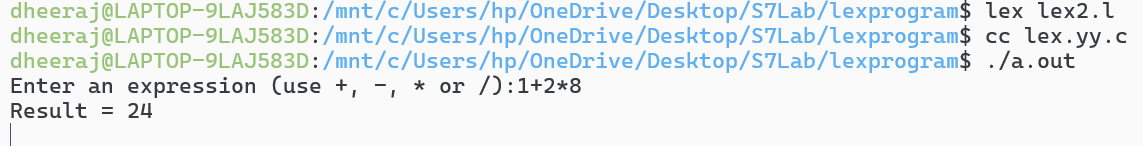
\includegraphics[width=\textwidth]{outs/exp10.png}

\newpage

\noindent
Name: Dheeraj A G\\
Roll No: 25

\vspace{0.15cm}

\noindent
\makebox[\textwidth]{\dotfill}

\vspace{0.05cm}

\begin{center}
    \textbf{ELIMINATION OF WHITE SPACES AND COMMENT LINES USING LEX PROGRAM}
\end{center}

\vspace{0.05cm}

\noindent
\makebox[\textwidth]{\dotfill}

\vspace{0.15cm}

\noindent
\underline{\textbf{PROGRAM}}

\vspace{0.1cm}

\begin{lstlisting}
%{
#include <stdio.h>
FILE *fp1, *fp2;
int flag = 0;
%}

WS [ \t]

%%
{WS}+ { }
"//" { flag = 1; }
"/*" { flag = 2; }
"\n" { if (flag == 1) flag = 0; }
"*/" { if (flag == 2) flag = 0; }
. { if (flag == 0) fprintf(fp2, "%s", yytext); }

%%

void main(int argc, char *argv[]) {
    fp1 = fopen(argv[1], "r");
    yyin = fp1;
    fp2 = fopen(argv[2], "w");
    yylex();
    fclose(fp1);
    fclose(fp2);
}

int yywrap() {
    return 1;
}
\end{lstlisting}

\vspace{0.15cm}

\noindent
\underline{\textbf{INPUT FILE (hello.c)}}

\vspace{0.1cm}

\begin{lstlisting}
#include <stdio.h>

int main() {
    // Single-line comment
    /*
     * Multi-line comment
     * Hello, World!
     */
    printf("Hello, World!\n");
    return 0;
}

\end{lstlisting}

\vspace{0.15cm}

\noindent
\underline{\textbf{OUTPUT FILE (out.c)}}

\vspace{0.1cm}

\begin{lstlisting}
#include<stdio.h>int main(){printf("Hello,World!\n");return 0;}
\end{lstlisting}

\vspace{0.15cm}

\noindent
\underline{\textbf{OUTPUT}}

\vspace{0.1cm}

\noindent
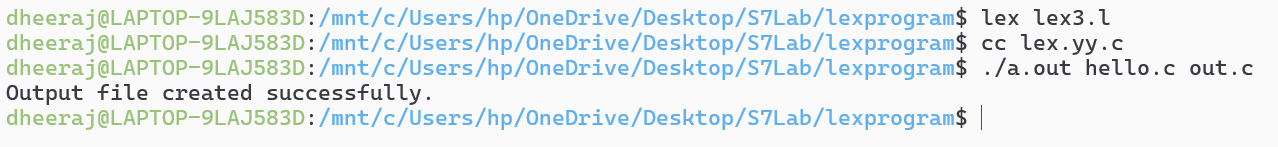
\includegraphics[width=\textwidth]{outs/exp11.png}

\newpage

\noindent
Name: Dheeraj A G\\
Roll No: 25

\vspace{0.15cm}

\noindent
\makebox[\textwidth]{\dotfill}

\vspace{0.05cm}

\begin{center}
    \textbf{SIMPLE CALCULATOR USING YACC PROGRAM}
\end{center}

\vspace{0.05cm}

\noindent
\makebox[\textwidth]{\dotfill}

\vspace{0.15cm}

\noindent
\underline{\textbf{PROGRAM}}

\vspace{0.1cm}

\begin{lstlisting}
%{
    #include <stdio.h>
    #include <ctype.h>

    int yylex(void);
    int yyerror(const char *message);
%}
%token NUMBER
%%
S: E '\n' { printf("Result = %d\n", $1); }
;
E: E '+' T { $$ = $1 + $3; }
 | T       { $$ = $1; }
;
T: T '*' F { $$ = $1 * $3; }
 | F       { $$ = $1; }
;
F: NUMBER  { $$ = $1; }
;
%%
int main(void)
{
    printf("Enter an expression: ");
    return yyparse();
}

int yylex(void)
{
    int ch = getchar();

    if (ch != EOF && isdigit((unsigned char) ch)) {
        ungetc(ch, stdin);
        scanf("%d", &yylval);
        return NUMBER;
    }

    return ch;
}

int yyerror(const char *message)
{
    (void) message;
    printf("Invalid expression!\n");
    return 0;
}
\end{lstlisting}

\vspace{0.15cm}

\noindent
\underline{\textbf{OUTPUT}}

\vspace{0.1cm}

\noindent
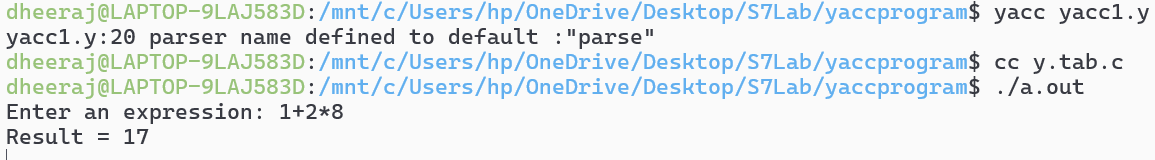
\includegraphics[width=\textwidth]{outs/exp12.png}

\newpage

\noindent
Name: Dheeraj A G\\
Roll No: 25

\vspace{0.15cm}

\noindent
\makebox[\textwidth]{\dotfill}

\vspace{0.05cm}

\begin{center}
    \textbf{ADVANCED CALCULATOR USING YACC PROGRAM}
\end{center}

\vspace{0.05cm}

\noindent
\makebox[\textwidth]{\dotfill}

\vspace{0.15cm}

\noindent
\underline{\textbf{PROGRAM}}

\vspace{0.1cm}

\begin{lstlisting}
%{
    #include <stdio.h>
    #include <ctype.h>

    int error = 0;

    int yylex(void);
    int yyerror(const char *message);
    int power(int base, int exponent);
%}
%token NUMBER
%%
S: S E '\n' {
        if (!error) {
            printf("Result = %d\n", $2);
        }
        error = 0;
    }
 | /* empty */
;
E: E '+' T { $$ = $1 + $3; }
 | E '-' T { $$ = $1 - $3; }
 | T       { $$ = $1; }
;
T: T '*' P { $$ = $1 * $3; }
 | T '/' P {
        if ($3 == 0) {
            printf("Error: division by zero\n");
            error = 1;
            $$ = 0;
        } else {
            $$ = $1 / $3;
        }
   }
 | P       { $$ = $1; }
;
P: U '^' P {
        if ($3 < 0) {
            printf("Error: negative exponent is not supported\n");
            error = 1;
            $$ = 0;
        } else {
            $$ = power($1, $3);
        }
   }
 | U       { $$ = $1; }
;
U: '-' U  { $$ = -$2; }
 | F      { $$ = $1; }
;
F: NUMBER { $$ = $1; }
 | '(' E ')' { $$ = $2; }
;
%%
int main(void){
    printf("Enter an expression: ");
    return yyparse();
}

int yylex(void){
    int ch = getchar();

    if (ch != EOF && isdigit((unsigned char) ch)) {
        ungetc(ch, stdin);
        scanf("%d", &yylval);
        return NUMBER;
    }

    return ch;
}

int yyerror(const char *message){
    (void) message;
    printf("Invalid expression!\n");
    error = 1;
    return 0;
}

int power(int base, int exponent){
    int result = 1;

    while (exponent > 0) {
        if (exponent % 2 == 1) {
            result *= base;
        }
        base *= base;
        exponent /= 2;
    }

    return result;
}
\end{lstlisting}

\vspace{0.15cm}

\noindent
\underline{\textbf{OUTPUT}}

\vspace{0.1cm}

\noindent
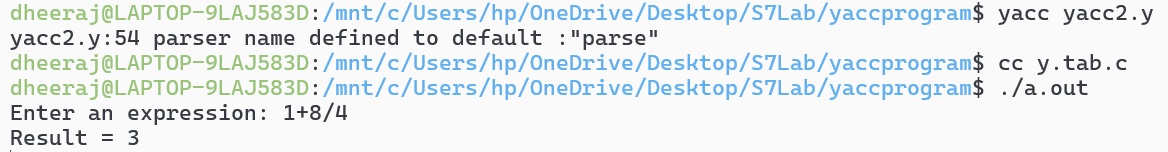
\includegraphics[width=\textwidth]{outs/exp13.png}

\newpage

\noindent
Name: Dheeraj A G\\
Roll No: 25

\vspace{0.15cm}

\noindent
\makebox[\textwidth]{\dotfill}

\vspace{0.05cm}

\begin{center}
    \textbf{VALIDATION OF IDENTIFIER USING YACC PROGRAM}
\end{center}

\vspace{0.05cm}

\noindent
\makebox[\textwidth]{\dotfill}

\vspace{0.15cm}

\noindent
\underline{\textbf{PROGRAM}}

\vspace{0.1cm}

\begin{lstlisting}
%{
#include <stdio.h>
#include <stdlib.h>
#include <ctype.h>

int yylex();
int yyerror(char *s);
%}
%token LETTER DIGIT
%%
L : S '\n' {printf("Valid Identifier\n");return 0;};

S : LETTER A
  | LETTER
  ;

A : LETTER A
  | DIGIT A
  | LETTER
  | DIGIT
  ;

%%

int yylex(){
    char c;

    c = getchar();

    if (isalpha(c))
        return LETTER;

    if (isdigit(c))
        return DIGIT;

    if (c == '\n')
        return '\n';

    return c;
}

int yyerror(char *s){
    printf("Invalid Identifier\n");
    return 0;
}

int main(){
    printf("Enter an identifier: ");
    yyparse();

    return 0;
}
\end{lstlisting}

\vspace{0.15cm}

\noindent
\underline{\textbf{OUTPUT}}

\vspace{0.1cm}

\noindent
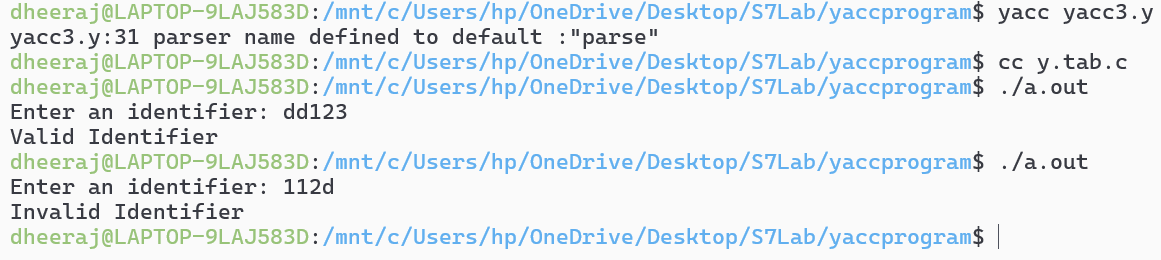
\includegraphics[width=\textwidth]{outs/exp14.png}

\newpage

\noindent
Name: Dheeraj A G\\
Roll No: 25

\vspace{0.15cm}

\noindent
\makebox[\textwidth]{\dotfill}

\vspace{0.05cm}

\begin{center}
    \textbf{INTERMEDIATE CODE GENERATION}
\end{center}

\vspace{0.05cm}

\noindent
\makebox[\textwidth]{\dotfill}

\vspace{0.15cm}

\noindent
\underline{\textbf{PROGRAM}}

\vspace{0.1cm}

\begin{lstlisting}
#include <stdio.h>
#include <string.h>
#include <ctype.h>

char stack[50];
int top = -1;

void push(char ch){
    stack[++top] = ch;
}

char pop(){
    return stack[top--];
}

int precedence(char ch){
    if (ch == '+' || ch == '-')
        return 1;

    if (ch == '*' || ch == '/')
        return 2;

    if (ch == '^')
        return 3;

    return 0;
}

void infixToPostfix(char infix[], char postfix[]){
    int i, j = 0;
    char ch;

    for (i = 0; infix[i] != '\0'; i++){
        ch = infix[i];

        if (isalnum(ch)){
            postfix[j++] = ch;
        }
        else if (ch == '('){
            push(ch);
        }
        else if (ch == ')'){
            while (top != -1 && stack[top] != '(')
            {
                postfix[j++] = pop();
            }

            if (top != -1)
                pop();
        }
        else{
            while (top != -1 && stack[top] != '(' && 
                    precedence(stack[top]) >= precedence(ch)){
                postfix[j++] = pop();
            }

            push(ch);
        }
    }
    while (top != -1){
        postfix[j++] = pop();
    }

    postfix[j] = '\0';
}

void generateTAC(char postfix[]){
    char stack[50][20];
    int top = -1;
    int i, temp = 1;

    char arg1[20], arg2[20], result[20];

    printf("\nTHREE ADDRESS CODE\n");

    for (i = 0; postfix[i] != '\0'; i++){
        if (isalnum(postfix[i])){
            stack[++top][0] = postfix[i];
            stack[top][1] = '\0';
        }
        else{
            strcpy(arg2, stack[top--]);
            strcpy(arg1, stack[top--]);

            sprintf(result, "t%d", temp++);

            printf("%s = %s %c %s\n",
                   result, arg1, postfix[i], arg2);

            strcpy(stack[++top], result);
        }
    }
}

void generateQuadruple(char postfix[]){
    char stack[50][20];
    int top = -1;
    int i, temp = 1;

    char arg1[20], arg2[20], result[20];

    printf("\nQUADRUPLE\n");

    printf("%-5s %-10s %-10s %-10s %-10s\n",
           "No.", "Operator", "Arg1", "Arg2", "Result");

    for (i = 0; postfix[i] != '\0'; i++){
        if (isalnum(postfix[i])){
            stack[++top][0] = postfix[i];
            stack[top][1] = '\0';
        }
        else{
            strcpy(arg2, stack[top--]);
            strcpy(arg1, stack[top--]);

            sprintf(result, "t%d", temp++);

            printf("%-5d %-10c %-10s %-10s %-10s\n",
                   temp - 1,
                   postfix[i],
                   arg1,
                   arg2,
                   result);
            strcpy(stack[++top], result);
        }
    }
}

void generateTriple(char postfix[]){
    char stack[50][20];
    int top = -1;
    int i, count = 0;

    char arg1[20], arg2[20];

    printf("\nTRIPLE\n");

    printf("%-5s %-10s %-10s %-10s\n",
           "No.", "Operator", "Arg1", "Arg2");


    for (i = 0; postfix[i] != '\0'; i++){
        if (isalnum(postfix[i])){
            stack[++top][0] = postfix[i];
            stack[top][1] = '\0';
        }
        else{
            strcpy(arg2, stack[top--]);
            strcpy(arg1, stack[top--]);

            printf("%-5d %-10c %-10s %-10s\n",
                   count,
                   postfix[i],
                   arg1,
                   arg2);

            sprintf(stack[++top], "(%d)", count);

            count++;
        }
    }
}

int main(){
    char infix[50];
    char postfix[50];

    printf("Enter infix expression: ");
    scanf("%s", infix);

    infixToPostfix(infix, postfix);

    printf("\nPostfix: %s\n", postfix);

    generateTAC(postfix);
    generateQuadruple(postfix);
    generateTriple(postfix);

    return 0;
}
\end{lstlisting}

\vspace{0.15cm}
\newpage
\noindent
\underline{\textbf{OUTPUT}}

\vspace{0.1cm}

\noindent
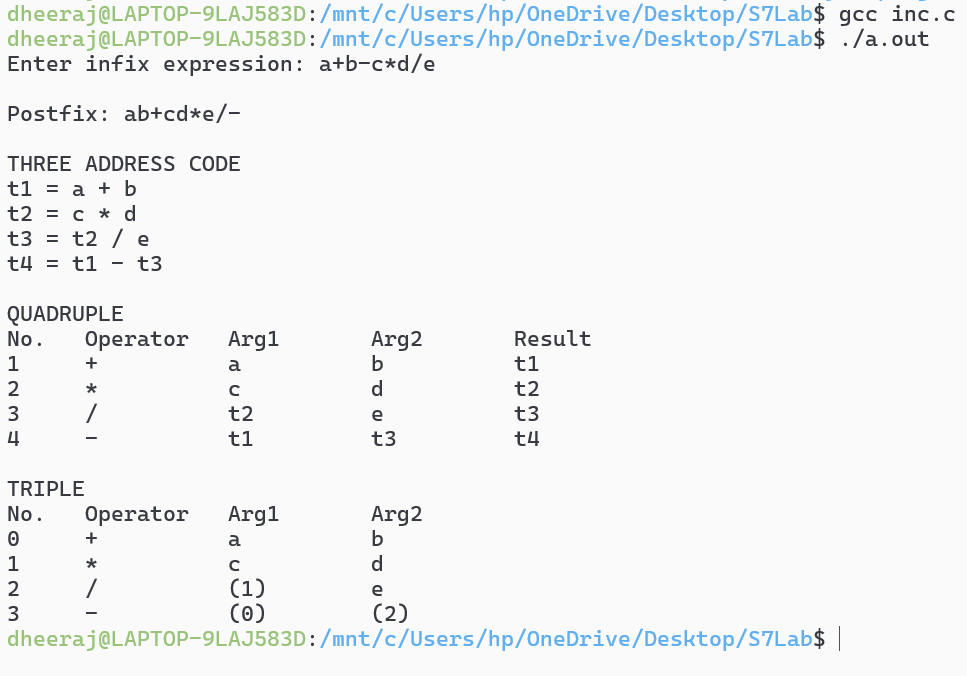
\includegraphics[width=\textwidth]{outs/exp15.png}

\newpage

\noindent
Name: Dheeraj A G\\
Roll No: 25

\vspace{0.15cm}

\noindent
\makebox[\textwidth]{\dotfill}

\vspace{0.05cm}

\begin{center}
    \textbf{ASSEMBLY CODE GENERATION}
\end{center}

\vspace{0.05cm}

\noindent
\makebox[\textwidth]{\dotfill}

\vspace{0.15cm}

\noindent
\underline{\textbf{PROGRAM}}

\vspace{0.1cm}

\begin{lstlisting}
#include <stdio.h>
#include <string.h>
#include <ctype.h>

char stack[100];
int top = -1;

void push(char ch){
    stack[++top] = ch;
}

char pop(){
    return stack[top--];
}

int precedence(char ch){
    if (ch == '+' || ch == '-')
        return 1;

    if (ch == '*' || ch == '/')
        return 2;

    return 0;
}

void infixToPostfix(char infix[], char postfix[]){
    int i, j = 0;
    char ch;

    for (i = 0; infix[i] != '\0'; i++){
        ch = infix[i];

        if (isalnum(ch)){
            postfix[j++] = ch;
        }
        else if (ch == '('){
            push(ch);
        }
        else if (ch == ')'){
            while (top != -1 && stack[top] != '(')
                postfix[j++] = pop();

            if (top != -1)
                pop();
        }
        else{
            while (top != -1 &&
                   stack[top] != '(' &&
                   precedence(stack[top]) >= precedence(ch))
            {
                postfix[j++] = pop();
            }

            push(ch);
        }
    }

    while (top != -1)
        postfix[j++] = pop();

    postfix[j] = '\0';
}

void generateAssembly(char postfix[], int start){
    int address = start;
    int i;
    char ch;

    printf("\nAddress\tInstruction\n");

    for (i = 0; postfix[i] != '\0'; i++){
        ch = postfix[i];

        if (isalnum(ch)){
            printf("%d\tMOV A,%c\n", address++, ch);
            printf("%d\tPUSH A\n", address++);
        }
        else{
            printf("%d\tPOP B\n", address++);
            printf("%d\tPOP A\n", address++);

            if (ch == '+')
                printf("%d\tADD B\n", address++);
            else if (ch == '-')
                printf("%d\tSUB B\n", address++);
            else if (ch == '*')
                printf("%d\tMUL B\n", address++);
            else if (ch == '/')
                printf("%d\tDIV B\n", address++);

            printf("%d\tPUSH A\n", address++);
        }
    }

    printf("%d\tPOP A\n", address++);
    printf("%d\tHLT\n", address++);
}

int main(){
    char infix[100];
    char postfix[100];
    int start;

    printf("Enter infix expression: ");
    scanf("%s", infix);

    printf("Enter starting address: ");
    scanf("%d", &start);

    infixToPostfix(infix, postfix);

    printf("\nPostfix expression: %s\n", postfix);

    generateAssembly(postfix, start);

    return 0;
}
\end{lstlisting}

\vspace{0.15cm}
\newpage
\noindent
\underline{\textbf{OUTPUT}}

\vspace{0.1cm}

\noindent
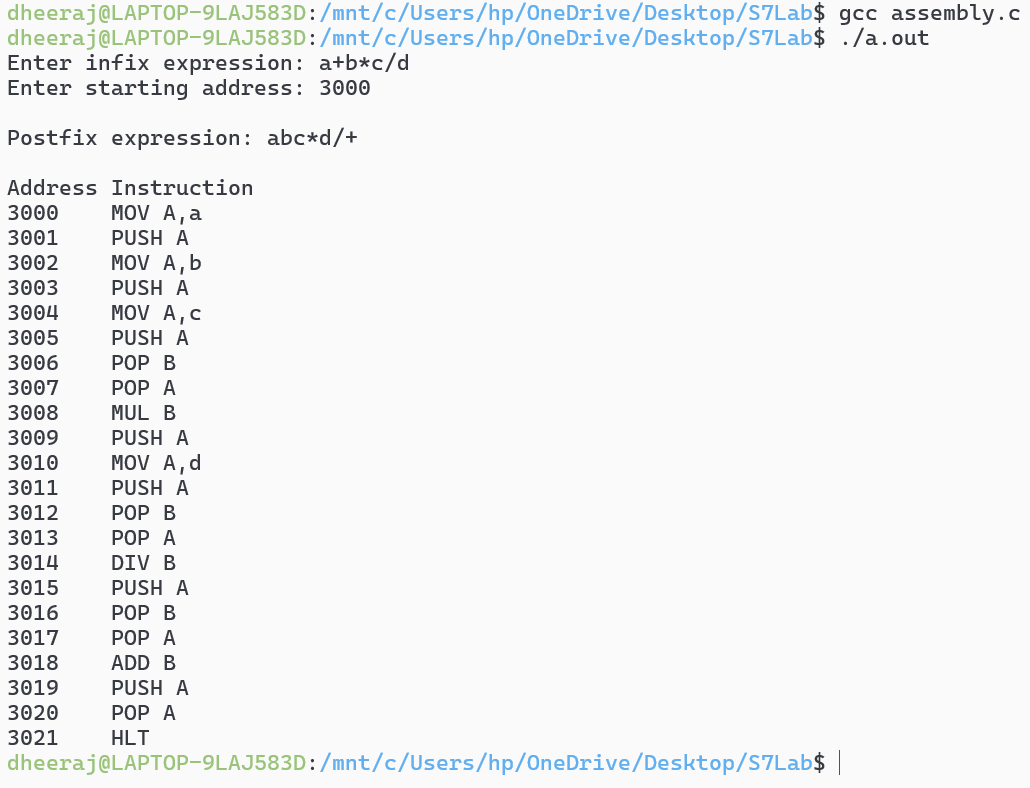
\includegraphics[width=\textwidth]{outs/exp16.png}

\end{document}
